\subsection{Applications}\label{sec:naysayer_apps}

The naysayer proof paradigm is generally applicable for proof systems with multi-round amplification, repetitive structure (e.g., multiple bilinear pairing checks~\cite{EPRINT:GabWilCio19}), or recursive reduction (e.g., Pietrzak's proof of exponentiation~\cite{ITCS:Pietrzak19b}). In this section, we highlight three example constructions of naysayer proofs.

\subsubsection{Merkle Commitments}\label{sec:merkle_naysayer}
\begin{figure*}[tbh]
    \centering
    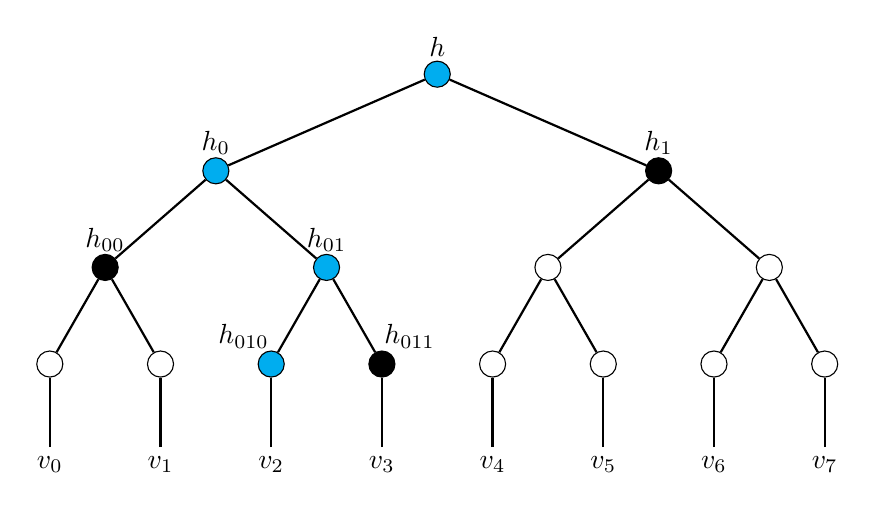
\begin{tikzpicture}[par/.style={sloped,fill=white,inner sep=-.4ex}]
    \tikzstyle{circ} = [circle, draw]
    \tikzstyle{path} = [circle, draw, fill=cyan]
    \tikzstyle{copath} = [circle, draw, fill=black]
        \node[path] (root) {};
        % level 1
        \node[path,below=3em,xshift=-8em] (l) at (root) {};
        \node[copath,below=3em,xshift=8em] (r) at (root) {};
        \draw[-,thick] (l) -- (root);
        \draw[-,thick] (r) -- (root);
        % level 2
        \node[copath,below=3em,xshift=-4em] (ll) at (l) {};
        \node[path,below=3em,xshift=4em] (lr) at (l) {};
        \draw[-,thick] (ll) -- (l);
        \draw[-,thick] (lr) -- (l);
        \node[circ,below=3em,xshift=-4em] (rl) at (r) {};
        \node[circ,below=3em,xshift=4em] (rr) at (r) {};
        \draw[-,thick] (rl) -- (r);
        \draw[-,thick] (rr) -- (r);
        % level 3
        \node[circ,below=3em,xshift=-2em] (lll) at (ll) {};
        \node[circ,below=3em,xshift=2em] (llr) at (ll) {};
        \draw[-,thick] (lll) -- (ll);
        \draw[-,thick] (llr) -- (ll);
        \node[path,below=3em,xshift=-2em] (lrl) at (lr) {};
        \node[copath,below=3em,xshift=2em] (lrr) at (lr) {};
        \draw[-,thick] (lrl) -- (lr);
        \draw[-,thick] (lrr) -- (lr);
        \node[circ,below=3em,xshift=-2em] (rll) at (rl) {};
        \node[circ,below=3em,xshift=2em] (rlr) at (rl) {};
        \draw[-,thick] (rll) -- (rl);
        \draw[-,thick] (rlr) -- (rl);
        \node[circ,below=3em,xshift=-2em] (rrl) at (rr) {};
        \node[circ,below=3em,xshift=2em] (rrr) at (rr) {};
        \draw[-,thick] (rrl) -- (rr);
        \draw[-,thick] (rrr) -- (rr);
        % leaves
        \node[below=3em] (0) at (lll) {$v_0$};
        \draw[-,thick] (0) -- (lll);
        \node[below=3em] (1) at (llr) {$v_1$};
        \draw[-,thick] (1) -- (llr);
        \node[below=3em] (2) at (lrl) {$v_2$};
        \draw[-,thick] (2) -- (lrl);
        \node[below=3em] (3) at (lrr) {$v_3$};
        \draw[-,thick] (3) -- (lrr);
        \node[below=3em] (4) at (rll) {$v_4$};
        \draw[-,thick] (4) -- (rll);
        \node[below=3em] (5) at (rlr) {$v_5$};
        \draw[-,thick] (5) -- (rlr);
        \node[below=3em] (6) at (rrl) {$v_6$};
        \draw[-,thick] (6) -- (rrl);
        \node[below=3em] (7) at (rrr) {$v_7$};
        \draw[-,thick] (7) -- (rrr);
        %%% labels
        % path
        \node[yshift=1em] at (root) {$h$};
        \node[yshift=1em] at (l) {$h_0$};
        \node[yshift=1em] at (lr) {$h_{01}$};
        \node[yshift=1em,xshift=-1em] at (lrl) {$h_{010}$};
        % copath
        \node[yshift=1em] at (r) {$h_1$};
        \node[yshift=1em] at (ll) {$h_{00}$};
        \node[yshift=1em,xshift=1em] at (lrr) {$h_{011}$};
    \end{tikzpicture}
    \caption{Each node in a Merkle tree consists of a hash of its children. The root $h$ is a commitment to the vector $(v_0, v_1, \dots, v_7)$ consisting of the leaves. To open the leaf at position 2, a prover provides the value $v_2$ and an opening proof $\pi$ consisting of the copath (black nodes) $(h_{011}, h_{00}, h_{1})$. The proof $\pi$ is checked by using its contents to recompute the root $h'$ starting with $v_2$, then checking that $h = h'$.
    In a naysayer proof system, the prover provides $\pi$ along with a ``verification trace'': the blue nodes $\com = (h_{010}, h_{01}, h_{0})$. A naysayer can point out an error at a particular point of the trace, e.g., $h_{01}$, which the naysayer verifier checks by computing a single hash, e.g., $H(h_{010}, h_{011}) \stackrel{?}{=} h_{01}$.}
    \label{fig:merkle-diagram}
\end{figure*}


\subsubsection{FRI Polynomial Commitment Scheme}\label{sec:fri_naysayer}

The FRI polynomial commitment scheme~\cite{EPRINT:BBHR18} is used as a building block in many non-interactive proof systems, including STARKs~\cite{STOC:BCGT13}.
Below, we describe only the parts of FRI relevant to our discussion. The FRI commitment to a polynomial $p(x)\in\mathbb{F}^{\leq d}[X]$ is the root of a Merkle tree with $\rho^{-1}d$ leaves. 
Each leaf is an evaluation of $p(x)$ on the set $L_0\subset\mathbb{F}$, where $\rho^{-1}d=\vert L_0\vert\ll\vert\FF\vert$, for $0<\rho<1$. We focus on the verifier's cost in the opening proof of the FRI polynomial commitment scheme as applied in the STARK IOP. Let $\delta$ be a parameter of the scheme such that $\delta\in(0,1-\sqrt{\rho})$. The prover sends the verifier $\log_2(\vert L_0\vert)$ messages. The FRI opening proof's verifier queries the prover's each message $\secpar/\log_2(1/(1-\delta))$ times to ensure $2^{-\secpar}$ soundness error. In each query, the verifier needs to check a Merkle-tree authentication path consisting of $\mathcal{O}(\log_2(\rho^{-1}d))$ hashes. Therefore, the overall STARK proof consists of $\mathcal{O}(\secpar\log_2(\rho^{-1}d)/\log_2(1/(1-\delta)))$ hashes. 

The overall STARK proof is invalid if any of the individual Merkle proofs is invalid. Therefore a straightforward naysayer proof $\pi^{\mathsf{FRI}}_{\nay}=(i,z_{i})$ need only point to the $i$th node in one of the Merkle proofs, where the hash values of the children nodes $x,y$ and their parent node $z\neq H(x,y)$ do not match in one of the incorrect Merkle authentication paths. The naysayer verifier only needs to compute a single hash evaluation $H(x,y)=z_{i}$ and check $z_{i}\neq z$. Thus, the naysayer proof for FRI has constant-size and can be verified in constant-time. 

\subsubsection{Post-quantum Signature Schemes}\label{sec:pqsig_naysayer}
With the advent of account abstraction~\cite{accountabstraction}, Ethereum users can define their own preferred digital signature schemes, including post-quantum signatures as recently standardized by NIST~\cite{CCS:BHKNRS19,TCHES:DKLLS18,NISTPQC:FALCON22}.
In all known schemes, %\joe{check this} 
post-quantum signatures or public keys are substantially larger than their classical counterparts.  Since post-quantum signatures are generally expensive to verify on-chain, they are prime candidates for the naysayer proof paradigm.

\paragraph{CRYSTALS-Dilithium~\cite{TCHES:DKLLS18}.} The verifier of this scheme checks that the following holds for signature $\sigma=(\mathbf{z},c)$, public key $\mathit{pk}=(\mathbf{A},\mathbf{t})$, and message $M$:
\begin{equation}\label{eq:crystals_verifier_check}
    \forall i: \lVert z_i\rVert_{\infty}\leq C\land \mathbf{A}\mathbf{z}-c\mathbf{t} = \mathbf{w} \land c=H(M\vert\vert \mathbf{w}),
\end{equation}
where $C$ is a constant, $\mathbf{A}\in R^{k\times l}_q$, and $\mathbf{z},\mathbf{t},\mathbf{w}\in R^{k}_q$ for the polynomial ring $R_q:=\mathbb{Z}_q[x]/(X^{256}+1)$. Notice that the checks in~\Cref{eq:crystals_verifier_check} are efficiently naysayable. In fact, the naysayer prover must show that the following holds: 
\begin{equation}\label{eq:crystals_naysayer_prover}
    \exists i: \lVert z_i\rVert_{\infty}>C\lor \mathbf{A}\mathbf{z}-c\mathbf{t} \neq \mathbf{w} \lor c\neq H(M\vert\vert \mathbf{w}).
\end{equation}
If the first check fails, then the naysayer prover shows an index $i$ for which the infinity norm of one of the polynomials in $\mathbf{z}$ is large. If the second check fails, then the naysayer prover can point to the $i$th row of the vector $\mathbf{w}$, where matrix-vector multiplication fails and verify only that row. Finally, if the last check fails, then the naysayer verifier just needs to recompute a single hash evaluation.

\paragraph{SPHINCS+~\cite{CCS:BHKNRS19}.} The signature verifier in SPHINCS+ checks several Merkle authentication proofs, requiring hundreds of hash evaluations. A constant-size and -time naysayer proof can be easily devised akin to the naysayer proof described in~\Cref{sec:fri_naysayer}. The naysayer prover simply points to the hash evaluation in one of the Merkle-trees where the signature verification fails. 

\subsubsection{Verifiable Shuffles}\label{sec:vshuffle_naysayer}
Verifiable shuffles are applied in many (blockchain) applications such as single secret leader election algorithms~\cite{AFT:Boneh20}, mix-nets~\cite{CACM:Chaum81}, cryptocurrency mixers~\cite{EPRINT:SNBB19}, and e-voting~\cite{USENIX:Adida08}. The state-of-the-art proof system for proving the correctness of a shuffle is due to Bayer and Groth~\cite{EC:BayGro12}. Their proof system is computationally heavy to verify on-chain as the proof size is $\mathcal{O}(\sqrt{n})$ and verification time is $\mathcal{O}(n)$, where $n$ is the number of shuffled elements. 

Most shuffling protocols (of public keys, re-randomizable commitments, or ElGamal ciphertexts) admit a succinct naysayer proof if the naysayer knows at least one of the shuffled elements. Let us consider the simplest case of shuffling public keys. We want to prove membership in the following  NP language:
\begin{equation}\label{eq:permlanguage}
    \mathcal{R}_{perm}:=\{(g^{\witness_i},g^{r\cdot \witness_{\sigma(i)}})^{n}_{i=1},g^r;\sigma,r\vert\ \forall i:\witness_i,r\in_{R}\mathbb{F}_p,g\in\mathbb{G},  \sigma\in_{R}\mathsf{Perm}(n)\}, 
\end{equation}
where $\mathsf{Perm}(n)$ is the set of all permutations $f:[n]\rightarrow[n]$.
Suppose the naysayer knows that for $j\in[n]$, the prover did not correctly include $g^{r\cdot \witness_j}$ in the shuffle. The naysayer can prove this by showing that $(g,g^{\witness_j},g^r,g^{r\cdot \witness_j})\in\mathcal{R}_{DH}\land g^{r\cdot \witness_j}\notin (\cdot,g^{r\cdot \witness_{\sigma(i)}})^n_{i=1}$, where $\mathcal{R}_{DH}$ is the language of Diffie-Hellman tuples. One can show that a tuple is a Diffie-Hellman tuple with a proof of knowledge of discrete logarithm equality~\cite{C:ChaPed92}. However, the naysayer must know the discrete logarithm $\witness_j$ to produce such a proof. Unlike our previous examples, which were publicly naysayable, this is a privately naysayable proof since the naysayer algorithm takes auxiliary input $\witness_j$. With the right data structure for the permuted list (e.g., a hash table), both of the above conditions can be checked in constant-time with a constant-size naysayer proof, resulting in exponential savings compared to directly verifying the original Bayer-Groth shuffle proof.

\subsubsection{zkVMs}

\noemi{Given an underlying zkVM, you can define a corresponding naysayer proof based on the $\mathsf{zkVM}.\vrfy$ circuit --- with the rise of zkVMs, should mention this. This is still ``application-specific'', since the naysayer proof depends on what zkVM is used (on its design/proof system). But in practice it's more ``general-purpose''. However, I think naysayer proofs are inherently application-specific since they rely on the structure of the verification circuit. But if we, as an area, start using only a few common verification circuits (e.g., adopting a few standard zkVMs), then the naysayer proof system can be reused.}

\noemi{update: not sure if it makes sense to talk about a $\mathsf{zkVM}.\vrfy$ circuit---they're generally just some proof system's verification procedure, e.g. the RISC Zero zkVM is running a STARK. Just talk about general naysaying by committing to a verification trace---and mention zkVMs somewhere as an example---then talk about particular languages where the verification trace is not needed because the structure is repetitive (i.e., conjunctions).}

\subsubsection{Evaluation}
We evaluate the asymptotic cost savings for the verifiers in the four examples discussed in \Cref{sec:fri_naysayer,sec:pqsig_naysayer,sec:vshuffle_naysayer}. Note that naysayer proofs allow an exponential speedup for the verifier for verifiable shuffles and a logarithmic speedup for the FRI polynomial commitment opening proof verifier, see~\Cref{tab:apps_table}. For CRYSTALS-Dilithium, we can only claim weakly efficient naysayer proofs, as there is no asymptotic gap in the complexity in certain branches of the signature verification circuit and the naysayer prover algorithm, cf.~\Cref{eq:crystals_verifier_check,eq:crystals_naysayer_prover}.

%------------------BEGIN Naysayer cost savings TABLE--------------
%-----------------------------------------
\begin{table}[tbh!]
   \centering
   \makebox[\linewidth]{
    \setlength{\belowbottomsep}{6pt}
    \begin{tabular}{l c c c c} 
    \toprule
     & \textbf{FRI Opening} & \textbf{CRYSTALS-D.} & \textbf{SPHINCS+}& \textbf{Shuffle proof} \\ [0.5ex] 
     \midrule
     $\pi$ storage & $\mathcal{O}(\secpar\log^2(d))\mathbb{H}$\ & $\mathcal{O}(\secpar)\FF$\  & $\mathcal{O}(\secpar)\FF$\  & $\mathcal{O}(\sqrt{n})\GG$\  \\ 
     $\vrfy(\pi)$ compute & $\mathcal{O}(\secpar\log^2(d))\mathbb{H}$\ & $\mathcal{O}(\secpar)\FF+1\mathbb{H}$\  & $\mathcal{O}(\secpar)\mathbb{H}$\  & $\mathcal{O}(n)\GG$\  \\\midrule
     $\pi_{nay}$ storage & $1\FF$\ & $1\FF\lor1\FF\lor1\FF$\  & $1\FF$\  & $2\GG+1\FF$\  \\
     ${\sf N}\vrfy(\pi_{nay})$ compute & $1\mathbb{H}$\ & $\mathcal{O}(\secpar)\FF\lor\mathcal{O}(\secpar)\FF\lor1\mathbb{H}$\  & $1\mathbb{H}$\  & $4\GG$\  \\
    \bottomrule
    \end{tabular}
    }
    \caption{Cost savings of the naysayer paradigm for the example applications in~\Cref{sec:naysayer_apps}. In FRI, let $deg(p(x))=d$. For the Bayer-Groth shuffle argument~\cite{EC:BayGro12}, we consider $n$ shuffled public keys (or ciphertexts). $\FF,\GG$ denotes field/group elements or field/group operations, respectively. $\mathbb{H}$ denotes hashing operations. }
    \label{tab:apps_table}
   \end{table}
   %--------------------END Naysayer cost savings TABLE--------------
   %-------------------------------------------------
   